% Chương 3: Phương pháp đề xuất

\chapter{Phương pháp đề xuất}

\section{Kiến trúc tổng thể hệ thống}

Hệ thống phát hiện xu hướng xã hội được xây dựng theo kiến trúc ba tầng:

\begin{enumerate}
    \item \textbf{Tầng thu thập dữ liệu (Producer)}: Thu thập nội dung từ ba nguồn TikTok, YouTube, và News thông qua các API và RSS feeds. Dữ liệu được chuẩn hóa và gửi vào Apache Kafka.

    \item \textbf{Tầng xử lý phân tích (Consumer)}: Đọc dữ liệu từ Kafka, xử lý qua pipeline tám giai đoạn sử dụng PySpark, phát hiện cụm xu hướng bằng HDBSCAN, phân tích bằng LLM, và lưu vào MongoDB.

    \item \textbf{Tầng giao diện người dùng (Dashboard)}: Cung cấp hai dashboard Streamlit - user dashboard để xem xu hướng, admin dashboard để quản lý hệ thống.
\end{enumerate}

\begin{figure}[H]
    \centering
    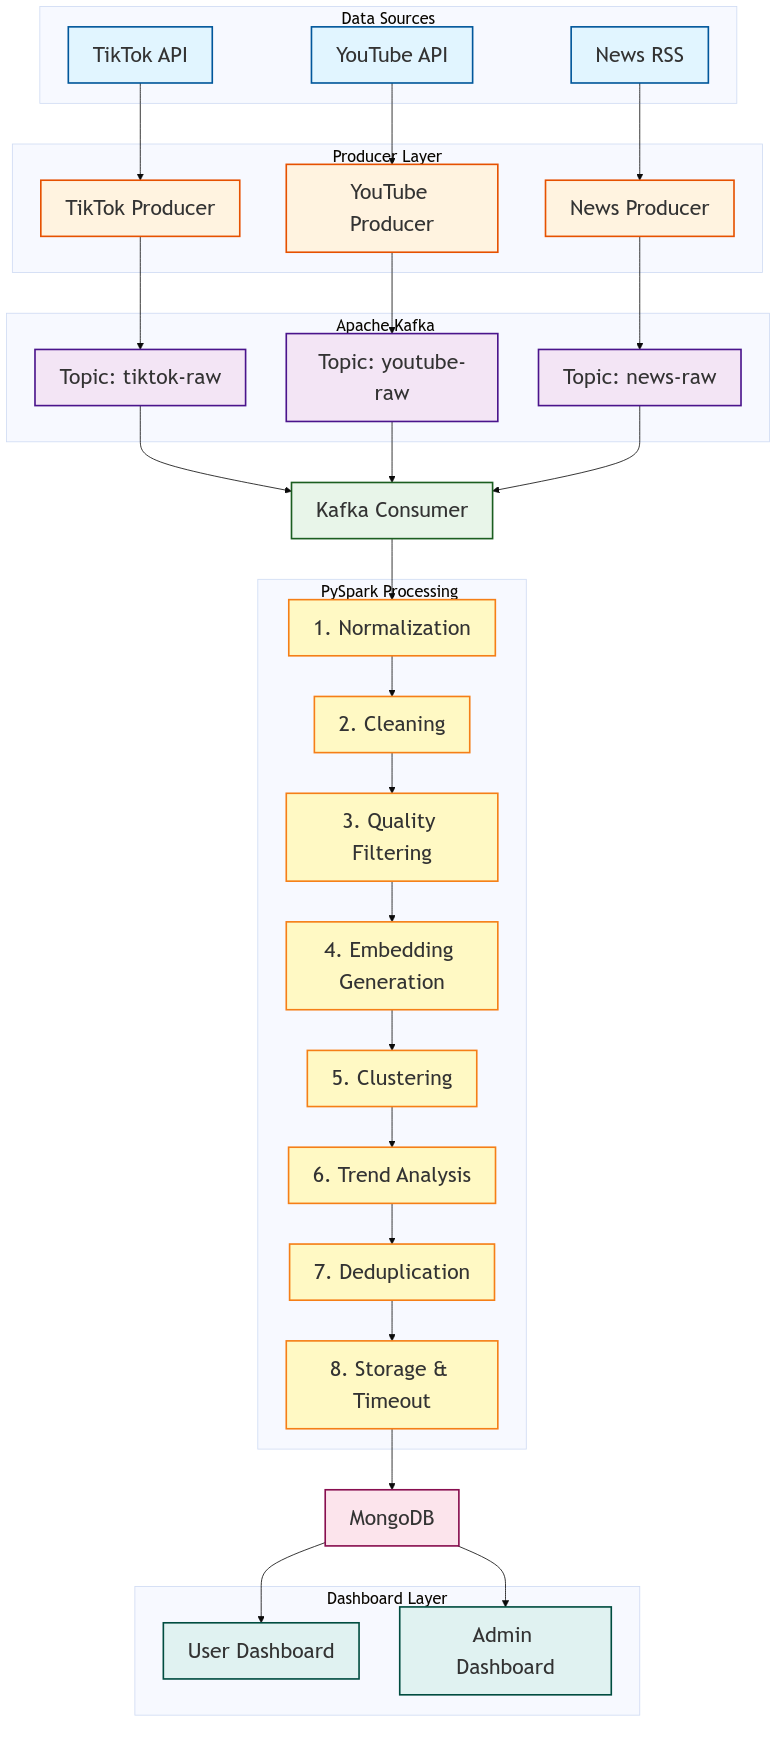
\includegraphics[width=0.7\textwidth]{images/architecture.png}
    \caption{Sơ đồ kiến trúc tổng thể hệ thống}
    \label{fig:architecture}
\end{figure}

\section{Pipeline xử lý tám giai đoạn}

Dữ liệu được xử lý qua 8 giai đoạn tuần tự:

\subsection{Giai đoạn 1: Chuẩn hóa (Normalization)}

Chuyển đổi dữ liệu từ ba nguồn khác nhau (TikTok, YouTube, News) về cấu trúc thống nhất với các trường:
\begin{itemize}
    \item content\_id: ID duy nhất của nội dung
    \item title: Tiêu đề nội dung
    \item description: Mô tả hoặc nội dung chính
    \item content: Nội dung đầy đủ (nếu có)
    \item author: Tác giả/tài khoản
    \item views, likes, comments, shares: Các chỉ số tương tác
    \item hashtags: Các hashtag liên quan
    \item source: Nguồn (tiktok/youtube/news)
    \item timestamp: Thời gian đăng
\end{itemize}

Hệ thống tạo trường \texttt{text\_for\_embedding} bằng cách nối title, description, và hashtags để chuẩn bị cho giai đoạn embedding.

\subsection{Giai đoạn 2: Làm sạch (Cleaning)}

Loại bỏ dữ liệu không hợp lệ:
\begin{itemize}
    \item Loại bỏ HTML tags, URLs, mentions
    \item Chuẩn hóa khoảng trắng, ký tự đặc biệt
    \item Xóa items thiếu title/description
    \item Xóa items có text quá ngắn (< 20 ký tự)
\end{itemize}

\subsection{Giai đoạn 3: Lọc chất lượng (Filtering)}

Loại bỏ spam, bot, và nội dung chất lượng thấp dựa trên:
\begin{itemize}
    \item Engagement rate: \(\text{likes/views} \geq 1\%\)
    \item Số người theo dõi tác giả: \(\geq 1000\) (nếu có)
    \item Độ dài nội dung: \(\geq 50\) ký tự
    \item Không chứa quá nhiều hashtags (giới hạn 20)
\end{itemize}

\subsection{Giai đoạn 4: Chuyển đổi vector (Embedding)}

Chuyển đổi text thành vector 1536 chiều bằng OpenAI \texttt{text-embedding-3-small} hoặc Gemini embedding model.

Công thức:
\[
    \text{embedding} = f(text\_for\_embedding)
\]

trong đó \(f\) là mô hình embedding, output là vector \(\mathbb{R}^{1536}\).

Hệ thống batch multiple items vào một request để tối ưu chi phí.

\subsection{Giai đoạn 5: Phân cụm (Clustering)}

Sử dụng HDBSCAN để phân cụm các embedding tương đồng:

\[
    \text{labels} = \text{HDBSCAN}(embeddings, \text{min\_cluster\_size}=15, \text{metric}=\text{euclidean})
\]

Hệ thống áp dụng two-pass clustering:
\begin{enumerate}
    \item Lần 1: HDBSCAN phân cụm, các items có label -1 (noise) được ghi nhận
    \item Lần 2: Gán các noise items vào cụm gần nhất nếu khoảng cách < 0.5 (cosine distance)
\end{enumerate}

Điều này giảm noise rate từ 10-15\% xuống còn 5-10\% mà vẫn giữ chất lượng cụm.

\subsection{Giai đoạn 6: Phân tích (Analysis)}

Phân tích từng cụm sử dụng LLM. Với mỗi cụm:
\begin{enumerate}
    \item Chọn top 10 items có engagement cao nhất
    \item Xây dựng prompt chứa title, description, stats của 10 items
    \item Gọi LLM (gpt-4.1-mini) để trích xuất:
          \begin{itemize}
              \item topic: Chủ đề chính (1-3 từ)
              \item summary: Tóm tắt 1-2 câu
              \item sentiment: positive/negative/neutral
              \item keywords: 5-10 từ khóa chính
              \item content\_type: entertainment/drama/commercial/social\_issue/dangerous
              \item risk\_level: safe/cautious/high\_risk/dangerous
              \item guidelines: Hướng dẫn cho marketer/social manager
          \end{itemize}
\end{enumerate}

Prompt được thiết kế để yêu cầu LLM trả về JSON có cấu trúc, dễ parse.

\subsection{Giai đoạn 7: Gộp xu hướng (Deduplication)}

Gộp xu hướng mới với xu hướng cũ (đã có trong MongoDB) nếu tương tự. Sử dụng chiến lược đa yếu tố:

\[
    \text{similarity\_score} = 0.4 \times \text{embedding\_sim} + 0.3 \times \text{keyword\_overlap} + 0.2 \times \text{time\_decay} + 0.1 \times \text{source\_sim}
\]

Trong đó:
\begin{itemize}
    \item embedding\_sim: Cosine similarity giữa embedding topic
    \item keyword\_overlap: Jaccard similarity giữa keywords
    \item time\_decay: Hệ số giảm theo thời gian (1.0 nếu cùng ngày, giảm dần)
    \item source\_sim: Độ tương đồng phân bố source
\end{itemize}

Nếu similarity\_score $\geq$ 0.5, gộp vào trend cũ. Ngược lại, tạo trend mới.

\subsection{Giai đoạn 8: Lưu trữ (Storage)}

Lưu xu hướng vào MongoDB collection \texttt{trends}. Tự động xóa các xu hướng cũ hơn 3 ngày để duy trì dữ liệu fresh.

Mỗi trend document chứa:
\begin{itemize}
    \item trend\_id, topic, summary, sentiment, keywords
    \item content\_type, risk\_level, guidelines
    \item sample\_items: Top 5 items có engagement cao
    \item stats: total\_views, total\_likes, avg\_engagement
    \item source\_counts: Số items từ mỗi source
    \item created\_at, updated\_at: Timestamps
\end{itemize}

\begin{figure}[H]
    \centering
    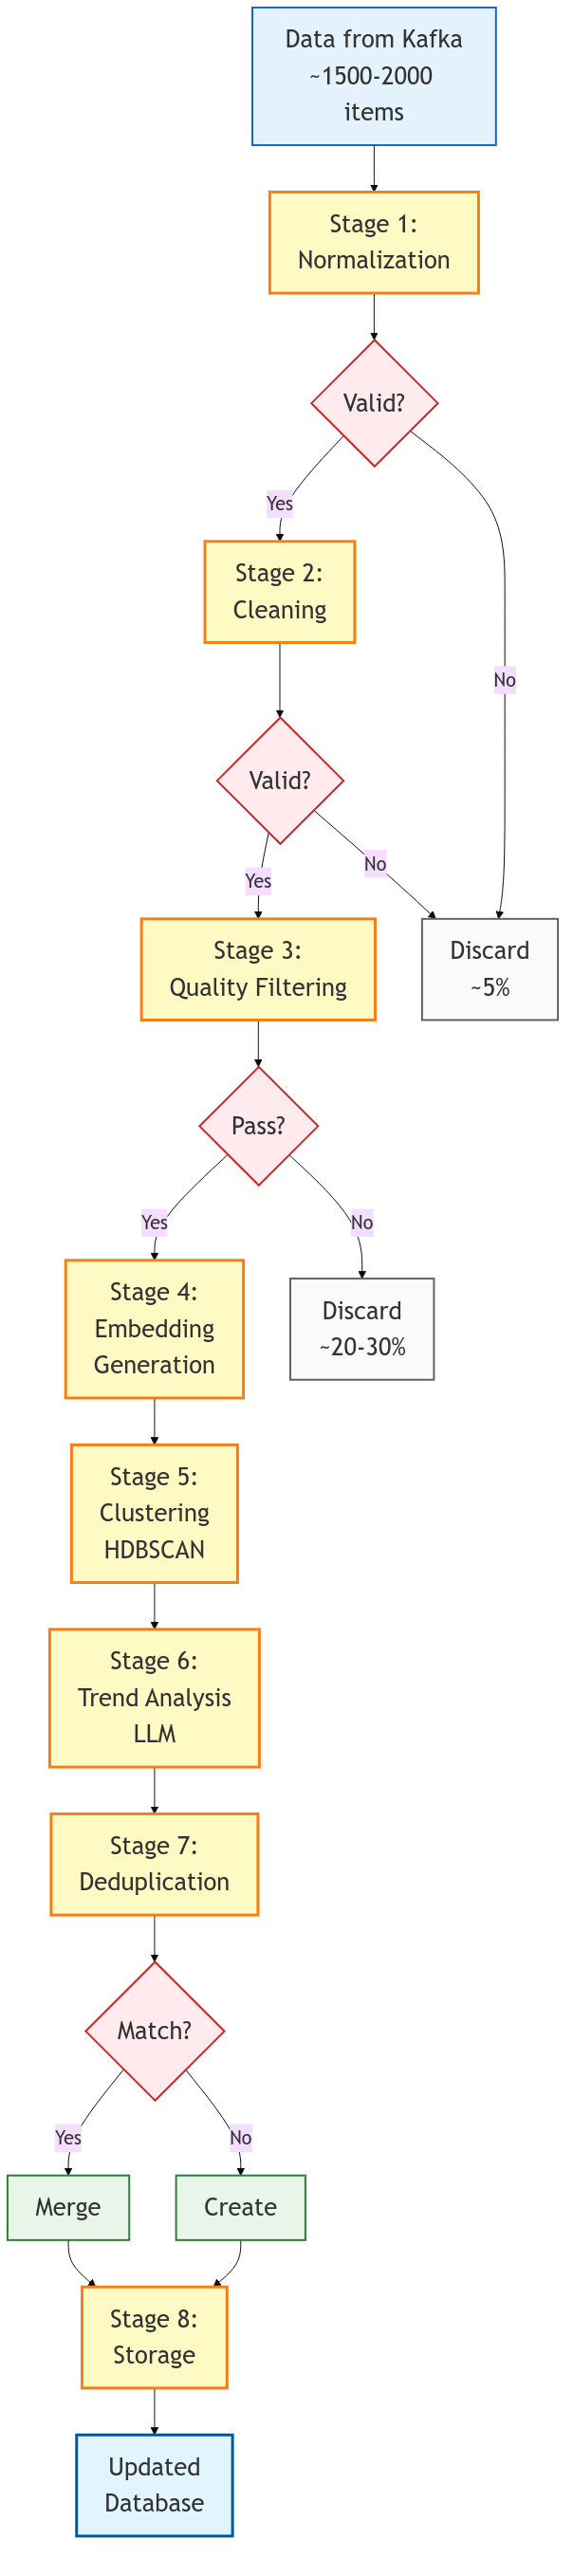
\includegraphics[width=0.3\textwidth]{images/pipeline.png}
    \caption{Sơ đồ pipeline xử lý 8 giai đoạn}
    \label{fig:pipeline}
\end{figure}

\section{Các công nghệ chính}

\subsection{Apache Kafka}

Kafka là nền tảng xử lý luồng sự kiện phân tán theo mô hình publish-subscribe. Trong đề tài này, Kafka làm hàng đợi tin nhắn giữa tầng thu thập và xử lý với ba topic (tiktok-raw, youtube-raw, news-raw), đảm bảo dữ liệu không bị mất khi xử lý thất bại.

\subsection{Apache Spark}

PySpark là framework xử lý dữ liệu lớn với tốc độ cao nhờ in-memory computing. Hệ thống dùng Spark để xử lý batch dữ liệu từ Kafka qua pipeline tám giai đoạn, với cấu hình local[*] để sử dụng tất cả core CPU.

\subsection{Vector Embeddings}

Vector embeddings biểu diễn văn bản dưới dạng vector trong không gian đa chiều, cho phép so sánh ngữ nghĩa. Hệ thống dùng OpenAI (text-embedding-3-small, 1536 chiều) để chuyển nội dung thành vector làm đầu vào cho phân cụm.

\subsection{HDBSCAN}

HDBSCAN là thuật toán phân cụm dựa mật độ, tự động xác định số cụm và xử lý tốt outliers. Hệ thống cấu hình: min\_cluster\_size=15, metric=``euclidean'', cluster\_selection\_method=``eom''.

\begin{figure}[H]
    \centering
    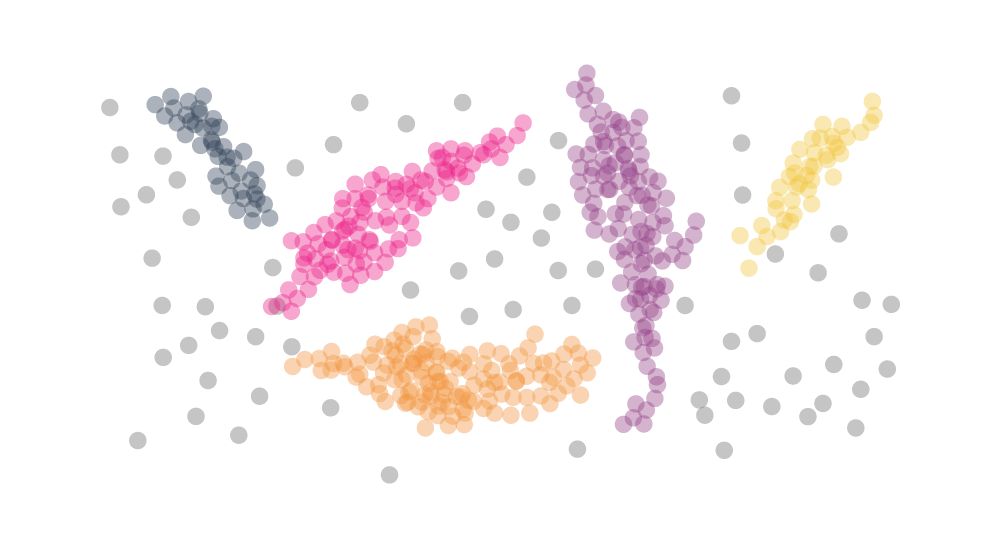
\includegraphics[width=0.8\textwidth]{images/hdbscan.png}
    \caption{Minh họa thuật toán HDBSCAN phân cụm dựa mật độ}
    \label{fig:hdbscan}
\end{figure}

\subsection{Large Language Models}

Hệ thống dùng LLM (gpt-4.1-mini) để phân tích, trích xuất topic, summary, sentiment, keywords, content\_type, risk\_level, guidelines từ mỗi cụm


\section{Tham số và giả định}

\subsection{Tham số chính}

\begin{table}[H]
    \centering
    \begin{tabular}{|l|l|l|}
        \hline
        \textbf{Tham số}      & \textbf{Giá trị}       & \textbf{Mô tả}                           \\
        \hline
        MIN\_CLUSTER\_SIZE    & 15                     & Kích thước tối thiểu cụm (HDBSCAN)       \\
        MIN\_ENGAGEMENT\_RATE & 1\%                    & Tỷ lệ engagement tối thiểu (likes/views) \\
        MIN\_AUTHOR\_FANS     & 1000                   & Số followers tối thiểu của tác giả       \\
        SIMILARITY\_THRESHOLD & 0.5                    & Ngưỡng gộp xu hướng (gộp xu hướng)       \\
        DEDUP\_WINDOW\_HOURS  & 24                     & Cửa sổ thời gian tìm trends cũ           \\
        TREND\_CLEANUP\_DAYS  & 3                      & Xóa trends cũ hơn N ngày                 \\
        EMBEDDING\_MODEL      & text-embedding-3-small & OpenAI embedding model                   \\
        LLM\_MODEL            & gpt-4.1-mini           & Model phân tích                          \\
        BATCH\_RUN\_INTERVAL  & 1 giờ                  & Chu kỳ chạy pipeline                     \\
        \hline
    \end{tabular}
    \caption{Các tham số chính của hệ thống}
    \label{table:parameters}
\end{table}

\subsection{Giả định}

\begin{enumerate}
    \item Giả định rằng nội dung từ các nguồn có thể so sánh được thông qua embedding vector
    \item Giả định rằng LLM có khả năng trích xuất chính xác chủ đề, cảm xúc, rủi ro từ các nội dung hỗn hợp
    \item Giả định rằng xu hướng tồn tại trong ít nhất 15 items trong một batch
    \item Giả định rằng engagement metrics có giá trị đại diện cho chất lượng và phạm vi của xu hướng
\end{enumerate}

